\section{Ziel}

\section{Theorie}
\label{sec:Theorie}

\cite{V308}

\subsection{Allgemeine Grundlagen zu Magnetfeldern} %"Magnetfelder von Spulen"?
Die magnetische Flussdichte $\symbf{B}$ wird durch die Permeabilität $\mu$ und die 
magnetische Feldstärke $\symbf{H}$ dargestellt. Es gilt die Beziehung 
\begin{equation*} 
    \symbf{B} = \mu \cdot \symbf{H}.
\end{equation*}
$\mu$ besteht dabei aus der Vakuum-Permeabilität $\mu_{0}$ und der relativen 
Permeabilität $\mu_{r}$, die von der Materie abhängt. 
Es gilt 
\begin{equation*} 
    \mu = \mu_{0} \cdot \mu_{r}.
\end{equation*}
\newline
%KURZE SPULE:
Die magnetische Flussdichte im Mittelpunkt einer Spule wird mit der Formel 
\begin{equation}
    \symbf{B}(x)= n \cdot \frac{\mu_{0} I}{2} \frac{R^2}{(R^2 +x^2)^{3/2}}\cdot \symbf{\hat{x}}
\end{equation}
beschrieben. 
Dabei ist $R$ der Radius des Rings und $n$ die Anzahl der Windungen.
%LANGE SPULE:
Bei einer langen Spule (Solenoid) ist die magnetische Feldstärke in der Mitte der 
Spule konstant. Außerhalb der Spule ist der magnetische Fluss inhomogen. 
Das innere Feld ist proportional zur Länge $l$ der Spule, zur Anzahl der Windungen 
$n$ und zum Strom $I$, der durch die Spule fließt. 
Es gilt die Beziehung
\begin{equation}
B = \mu_{r} \mu_{0} \frac{n}{l} I.
\end{equation}
%SPULENRING:
Wird dieser Solenoid zu einem Ring mit Radius $r_{R}$ gebogen, verschwinden die 
Randeffekte und das Feld außerhalb des Rings wird null. 
Im Inneren gilt
\begin{equation}
B = \mu_{r} \mu_{0} \frac{n}{2\pi r_{R}} I.
\end{equation}

\subsection{Magnetfeld eines Spulenpaares}
Ein Helmholtz-Spulenpaar hat ein homogenes Magnetfeld im Innern der zwei Ringe %Spulen statt Ringe
(s. Abb \ref{fig:helmholtz}). Der Abstand der Spulen entspricht den Radien der
Spulen.
Die magnetische Flussdichte im Mittelpunkt des Spulenpaares ist durch 
\begin{equation}
B(0)= B_{n}(x) + B_{n}(-x) = 2n \frac{\mu_{0} I R^2}{(R^2 + x^2)^3/2} %mal 2n oder n???????????
\end{equation}
gegeben.
\begin{figure}
    \centering
    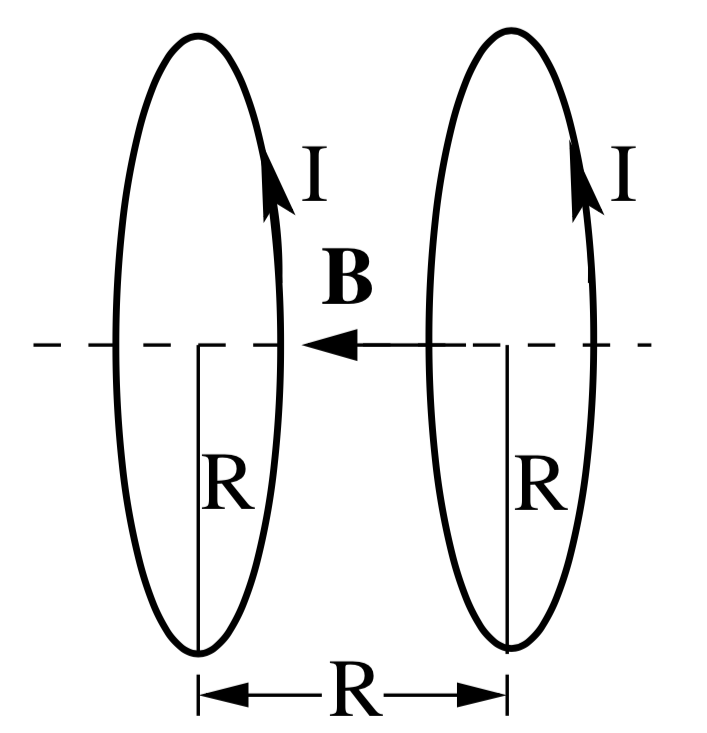
\includegraphics[width=6cm,hight=8cm]{build/Helmholtz.png}
    \caption{Aufbau eines Helmholtz-Spulenpaares. Der Abstand der Spulen
    entspricht den Radien der Spulen.}
    \label{fig:helmholtz}
\end{figure}

\subsection{Ferromagnetismus und die Hysteresekurve}
Ferromagnetische Materialien besitzen ohne äußere Magnetfelder ein permanentes 
magnetisches Moment. Sie richten sich in einzelnen Bereichen parallel zueinander aus. 
Man nennt diese Bereiche Weiß'sche Bezirke. Im unmagnetischen Zustand ist die 
Ausrichtung der Bereiche statistisch verteilt. Ein äußeres Magnetfeld sorgt für eine 
Änderung der Richtung der magnetischen Momente und vergrößert somit die Weiß'schen 
Bereiche. 
\newline
Die relative Permeabilität $\mu_{r}$ ist in ferromagnetischen Materialien sehr hoch 
und ist nicht mehr linear proportional zur magnetischen Flussdichte. 
Die Abhängigkeit kann durch eine Hysteresekurve dargestellt werden.
%B wird gegen H aufgetragen. Bei uns I?
In der Kurve lassen sich verschiedene markante Punkte erkennen. 
Ohne äußeres Magnetfeld gilt $B = H = 0$. Wird ein Magnetfeld angelegt, steigt die 
Magnetisierung an, bis ein Sättigungswert $B_{S}$ bei $H_{S}$ erreicht wird. Der 
Kurvenverlauf dorthin wird Neukurve genannt. 
Wird das äußere Magnetfeld verringert, bilden sich Bereiche mit entgegengesetzer 
Magnetisierung. So bleibt, wenn das äußere Magnetfeld abgeschaltet wird, eine 
Restmagnetisierung $B_{r}$, genannt Remanenz, bestehen. 
Ein Gegendfeld $H_{c}$, genannt Koerzitivkraft, kann diese Ausrichtungen wieder 
aufheben, sodass die magnetische Flussdichte Null wird. Wenn dieses Feld noch weiter 
erhöht wird, wird die Magnetisierung %Magnetisierung oder magnetische Flussdichte? Magnetisierung ist doch schon negativ gewesen.
in dem Stoff negativ und erreicht den Sättigungswert $-B_{S}$. Wird das äußere 
Magnetfeld wieder umgekehrt, entsteht eine zum Ursprung punktsymmetrische Kurve, welche
Hysteresekurve genannt wird. Hysteresekurven verschiedener Stoffe unterscheiden sich je
nach Materialeigenschaften in der Schärfe bzw. Breite. 
\begin{figure}
    \centering
    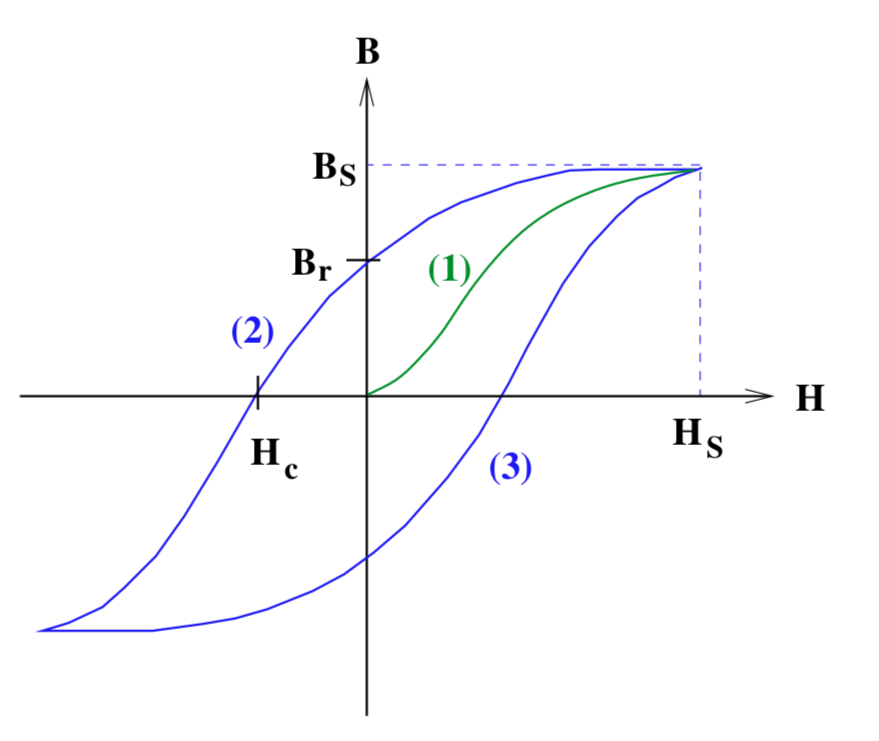
\includegraphics[width=10cm,hight=10cm]{build/Hysteresekurve.png}
    \caption{Allgemeine Hysteresekurve. Eingezeichnet sind der Sättigungswert $B_{S}$
    sowie $H_{S}$, die Remanenz $B_{r}$ und die Koerzitivkraft $H_{c}$.}
\end{figure}
%\newline
% Die differentielle Permeabilität $\mu_{diff}$ ist als
% \begin{equation}
% \mu_{diff} = \frac{1}{\mu_{0}} \frac{dB}{dH}
% \end{equation}
% definiert.